\begin{frame}{\ft{About}}

	\pdfpageheight 30cm

        \begin{annotatedFigure}
            {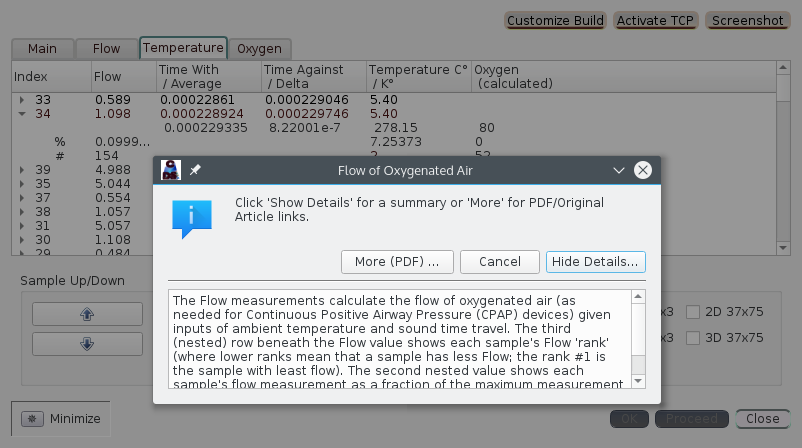
\includegraphics[scale=1]{about.png}}
            
  \node [text width=12cm,align=justify,fill=logoCyan!20, draw=logoBlue, 
  draw opacity=0.5,line width=1mm, fill opacity=0.9]
   at (0.58,0.76){\textbf{Context menus also allow users to 
   obtain information and explanations about individual parts of the 
   data set, such as individual statistical parameters.  In this 
   screenshot, the user has right-clicked on a data column and 
   chosen a context menu action which shows, via a dialog box, 
   a precis of the quantities represened in that column and their 
   significance for the data set as a whole.}};

            \annotatedFigureBox{0.2,0.12}{0.812,0.645}{1}{0.81,0.645}%            
      %      \annotatedFigureBox{0.222,0.284}{0.3743,0.4934}{B}{0.3743,0.4934}%tr
      %      \annotatedFigureBox{0.555,0.784}{0.6815,0.874}{C}{0.555,0.784}%bl
      %      \annotatedFigureBox{0.557,0.322}{0.8985,0.5269}{D}{0.8985,0.5269}%tr
  
        \end{annotatedFigure}

\end{frame}
